\section{The LZ Detector}
\par
The LUX-ZEPLIN (LZ) experiment is a second-generation direct detection dark matter experiment, named from it's predecessor LUX, and the ZEPLIN series of experiments which pioneered xenon phase detectors.

The LZ experiment has been primarily designed for the detection WIMP dark matter candidates described in XXX. 
This is primarily done through a dual-phase Time-Project Chamber (TPC).

\par
The LZ experiment is a multi-detector system, which work together to increase the sensitivity to dark matter candidates.
A cut through of the LZ experiment is shown in Figure 

\begin{figure}
    \centering
    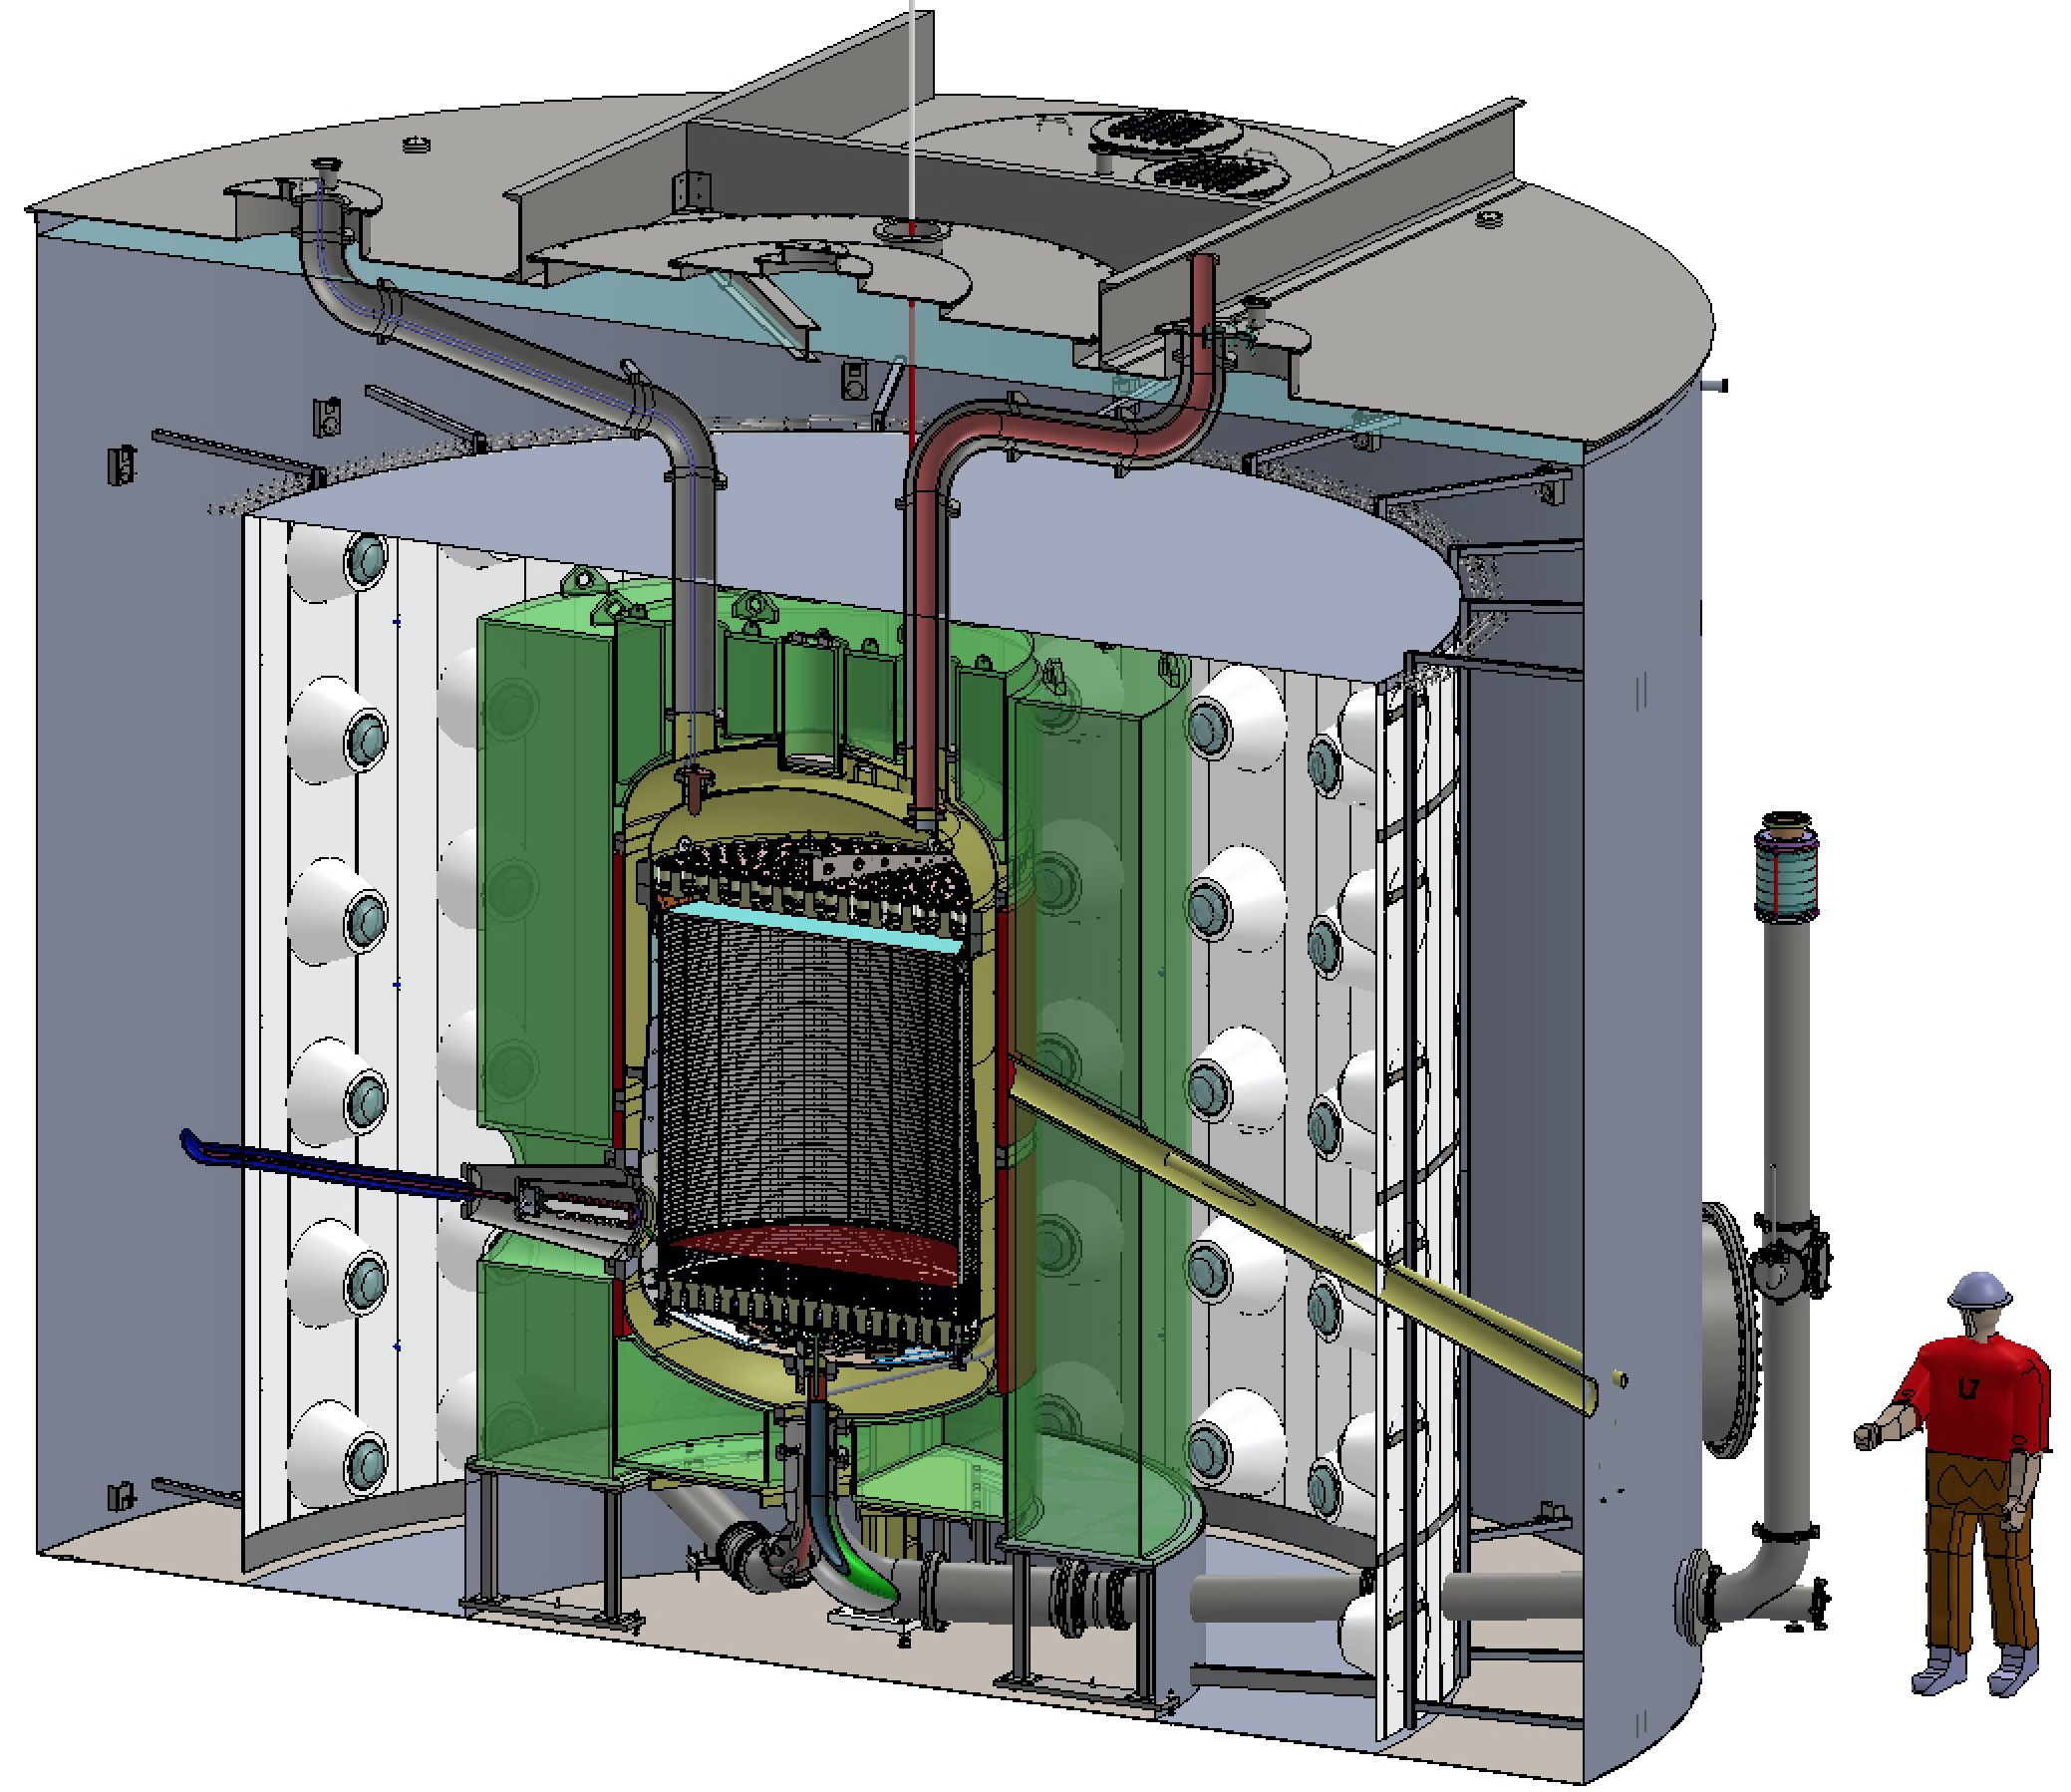
\includegraphics[width=\linewidth]{Figures/LZ/LZ_Cut_CAD.jpg}
    \caption{Cross-Section of the LZ experiment. Figure from Ref \cite{LZ_TechnicalDesignReview_ref}}
    \label{fig:LZ_Cut_CAD}
\end{figure}



\par
In the remainder of this chapter, the design and construction of the LZ experiment are detailed with particular emphasis on the TPC, Skin and OD which are relevant for the remainder of this thesis. 
It should be noted that the design is detailed in significant more detail in the Technical Design Review \cite{LZ_TechnicalDesignReview_ref}.

\subsection{TPC}
\par
At the centre of the LZ experiment is the TPC.
It's purpose is the production of S1 and S2 light from particle interactions as previously described in Section XXX.
\par
The TPC is comprised of 2 arrays of photo-multiplier tubes (PMTs); one at the top and one at the bottom, which serve to collect the light from any particle interaction which happens within the TPC volume.
The wall of the TPC is made from PTFE.
\par
The TPC is filled almost entirely with liquid Xenon, with the exception being the gas Xenon pocket just under the top PMT array.

\subsection{Skin}
\par


\subsection{OD}
\par
Surrounding OCV is the outer-detector (OD).
It consists of 10-segments of acrylic tanks (something about UV), which fit around the OCV as shown in Figure XXX.
Together these provide near 4$\pi$ coverage about the OCV.

\par
The OD tanks are filled with a linear akylbenze (LAB) doped with 0.1\% natural Gadolinium (by mass) - which together are refereed to as the Gadolinium Liquid Scintillator (GdLS).



\par



\subsubsection{Design Changes}
\par
During the installation phase of the Acrylic tanks about the OCV, the curvature of the top Acrylic tanks were significantly different to that of the OCV, as such, the top 2 acrylic tanks could not be placed around the 

\par


\subsection{Water}

\subsection{Underground}

\subsection{Backgrounds}

\subsection{Calibrations}
\par
In order for the above experiment to work and have understandable results, a set of calibrations are required to characterise the; energy scale, energy threshold and detection efficiency.
In this section the calibration systems are explained, along with the different sources that are deployable.
A summary of the sources used prior to SR1 are shown in Table XXX. 
Additional sources planed are outlined in the LZ Technical Design Review \cite{LZ_TechnicalDesignReview_ref}

\begin{table}[!htbp]
    \centering
    \begin{tabular}{c|c|c|c}
    \hline
    Isotope       & Interacting particle         & Purpose                    & Deployment \\
    \hline
    ${}^{83m}Kr $ & beta/gamma, 32.1 keV/9.4 keV & TPC (x,y,z)                & Internal  \\
    ${}^{131m}Xe$ & 164 keV gamma                & TPC (x,y,z), Xe skin       & Internal  \\ 
    ${}^{220}Rn $ & various alphas               & xenon skin                 & Internal  \\
    $AmLi       $ & (alpha, n)                   & NR band                    & CSD       \\
    ${}^{252}Cf $ & spontaneous fission          & NR efficiency              & CSD       \\
    ${}^{57}Co  $ & 122 keV gamma                & Xe skin threshold          & CSD       \\
    ${}^{228}Th $ & 2.615 MeV gamma              & OD energy scale            & CSD       \\
    ${}^{22}Na  $ & back-to-back 511 keV gamma’s & TPC and OD sync            & CSD       \\
    ${}^{88}Y Be$ & 152 keV neutron low-energy   & NR response                & External  \\
    $DD         $ & 2,450 keV neutron            & NR light and charge yields & External  \\
    $DD         $ & 272 keV neutron              & NR light and charge yields & External
    \end{tabular}
    \caption{LZ calibration sources that were used for calibration prior to the first science run along with the calibration purpose and deployment method. Table adapted from \cite{LZ_TechnicalDesignReview_ref}.}
    \label{tab:LZ_Used_Calibration_Sources}
\end{table}


\subsubsection{Internal}
\par

\subsubsection{Calibration Source Tubes}
\par

\subsubsection{External}
\par
External sources are sources which are outside of the OCV.

\section{Detector Status}
\par
At the time of writing this thesis, the LZ experiment construction has been completed and the first Science Run completed???
However, it should be noted that due to various construction delays, the calibration and comissioning campaigns were reduced in scope which has implications for the 

